This Exercise has been completed in the attached Jupyter Notebook titled: "integration"
Just in case, the resulting plots are given here. Note that there are two graphs to show that they follow $ln(x)$, because it is hidden behind the approximated function with step length $0.01$\\
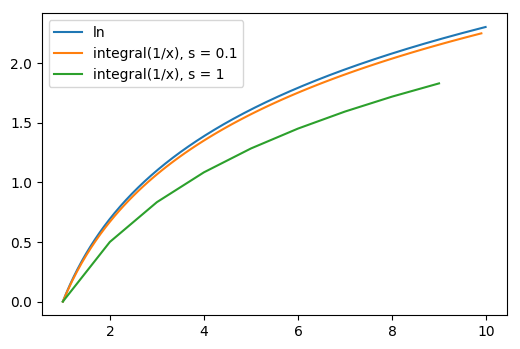
\includegraphics[width=0.5\linewidth]{lnnosmall}
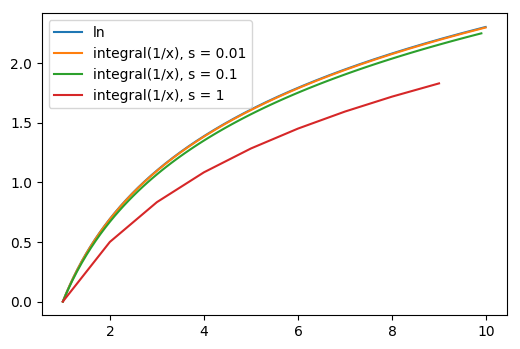
\includegraphics[width=0.5\linewidth]{lnwithsmall}
The most important bit of code is the following, which actually calculates the integral up to a given $x$:
\begin{verbatim}
def integrate(x, s):
    values = np.arange(1.0, x, s)
    retVal = [0]*len(values)
    for i in range(1, len(values)):
        if (i>0):
            retVal[i] = retVal[i-1] + s/values[i]
        else:
            retVal[i] = 0
    return retVal
\end{verbatim}